\subsection{Chapter 12 - Simple harmonic motion}

\subsubsection{Overview}\label{chapter:simpleharmonicmotion}

In this chapter, we look at oscillating systems that undergo ``simple harmonic motion'', such as the motion of a mass attached to a spring. Many systems in the physical world, such as an oscillating pendulum, can be described by the same mathematical formalism that describes the motion of a mass attached to a spring.

\begin{framed}
\textbf{Learning Objectives}\\
\begin{itemize}
\item Understand how to model the position, velocity, and acceleration of a mass attached to a spring.
\item Understand the conditions under which a system undergoes simple harmonic motion.
\item Understand how to model the motion of a pendulum when it undergoes simple harmonic motion.
\end{itemize}
\end{framed}

\begin{framed}
\textbf{Think About It}\\
What do the motion of a mass attached to a spring, a cork bobbing in the water, and a pendulum have in common?
\end{framed}

\subsubsection{The motion of a spring-mass system}

As an example of simple harmonic motion, we first consider the motion of a block of mass $m$ that can slide without friction along a horizontal surface. The mass is attached to a spring with spring constant $k$ which is attached to a wall on the other end. We introduce a one-dimensional coordinate system to describe the position of the mass, such that the $x$ axis is co-linear with the motion, the origin is located where the spring is at rest, and the positive direction corresponds to the spring being extended. This ``spring-mass system'' is illustrated in Figure~\ref{fig:simpleharmonicmotion:spring}.

\begin{figure}[!htbp]
\centering
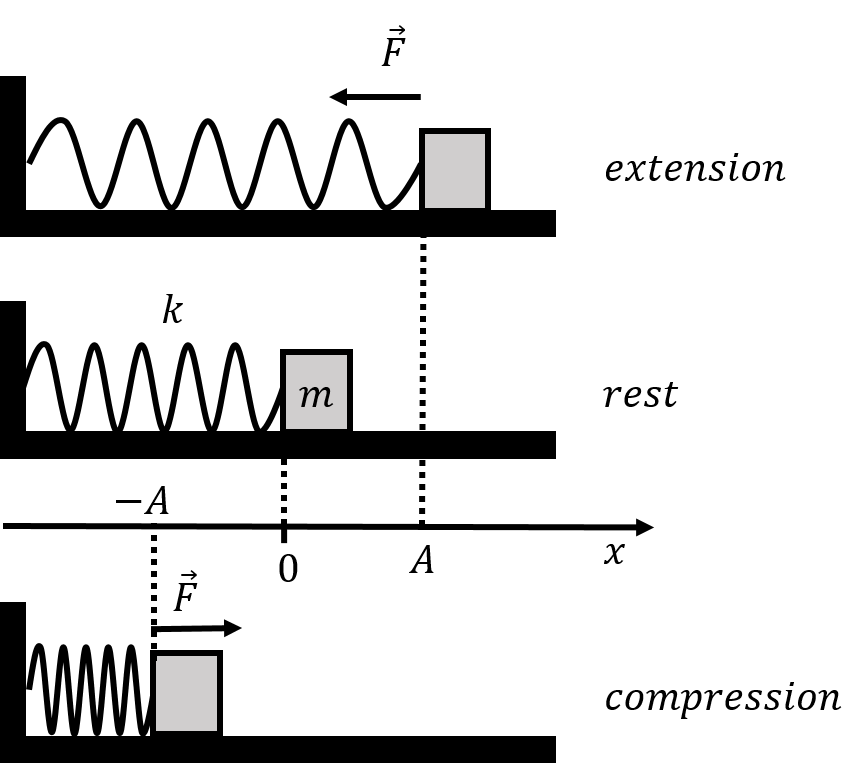
\includegraphics[width=0.6\linewidth]{files/spring-e6d47243885eb7276547802f935f9caf.png}
\caption[]{A horizontal spring-mass system oscillating about the origin with an amplitude $A$.}
\label{fig:simpleharmonicmotion:spring}
\end{figure}

We assume that the force exerted by the spring on the mass is given by Hooke's Law:
\begin{equation}
\vec F = -kx \hat x
\end{equation}
where $x$ is the position of the mass. The only other forces exerted on the mass are its weight and the normal force from the horizontal surface, which are equal in magnitude and opposite in direction. Therefore, the net force on the mass is the force from the spring.

As we saw in Section Section~\ref{sec:potentialecons:ediagrams}, if the spring is compressed  (or extended) by a distance $A$ relative to the rest position, and the mass is then released, the mass will oscillate back and forth between $x=\pm A$\footnote{As long as there is no friction to reduce the mechanical energy of the mass.}, which is illustrated in Figure~\ref{fig:simpleharmonicmotion:spring}. We call $A$ the ``amplitude of the motion''. When the mass is at $x=\pm A$, its speed is zero, as these points correspond to the location where the mass ``turns around''.

\paragraph{Description using energy}

We can describe the motion of the mass using energy, since the mechanical energy of the mass is conserved. At any position, $x$, the mechanical energy, $E$, of the mass will have a term from the potential energy, $U$, associated with the spring force, and kinetic energy, $K$:
\begin{equation}
E = U + K =\frac{1}{2}kx^2 + \frac{1}{2}mv^2
\end{equation}
We can find the mechanical energy, $E$, by evaluating the energy at one of the turning points. At these points, the  kinetic energy of the mass is zero, so $E=U(x=A)=1/2kA^2$. We can then write the expression for mechanical energy as:
\begin{equation}
\boxed{\frac{1}{2}kx^2 + \frac{1}{2}mv^2 = \frac{1}{2}kA^2}
\end{equation}
We can thus always know the speed, $v$, of the mass at any position, $x$, if we know the amplitude $A$:
\begin{equation}
v(x) = \sqrt{\frac{k(A^2-x^2)}{m}}
\end{equation}

\begin{framed}
\textbf{Checkpoint}\\
If you double the amplitude of the motion of a mass attached to a spring, its maximum speed will be:

\begin{enumerate}
\item double.
\item $\sqrt 2$ times greater.
\item the same.
\item halved.
\end{enumerate}

\begin{framed}
\textbf{Answer}\\
\begin{enumerate}
\item
\end{enumerate}
\end{framed}
\end{framed}

\paragraph{Kinematics of simple harmonic motion}

We can use Newton's Second Law to obtain the position, $x(t)$, velocity, $v(t)$, and acceleration, $a(t)$, of the mass as a function of time. The $x$ component of Newton's Second Law for the mass attached to the spring can be written:
\begin{equation}
\sum F_x = -kx = ma
\end{equation}
We can write the acceleration in Newton's Second Law more explicitly as the second derivative of the position, $x(t)$, with respect to time. If we do this, we can see that Newton's Second Law for the mass attached to the spring is a differential equation for the function $x(t)$ (we call it an ``equation of motion''):
\begin{equation}
\label{eq:simpleharmonicmotion:shmspring}
ma &= -kx\nonumber\\
m\frac{d^2x}{dt^2} &= -kx\nonumber\\
\therefore \frac{d^2x}{dt^2} &= -\frac{k}{m}x
\end{equation}
We want to find the position function, $x(t)$. Equation \{{\textbackslash}ref\{eq:simpleharmonicmotion:shmspring\}\} tells us that the second derivative of $x(t)$ with respect to time must equal the negative of the $x(t)$ function multiplied by a constant, $k/m$. Without having taken a course on differential equations, it might not be obvious what the function $x(t)$ could be. Several, equivalent functions can satisfy this equation. One possible choice, which we present here as a guess, is{\textbackslash}footnote\{Other possible guesses that work are $A \sin(\omega t + \phi)$, and $x(t) = A\cos(\omega t) + B\sin(\omega t)$.\}:
\begin{equation}
\boxed{x(t) = A \cos(\omega t + \phi)}
\end{equation}
where $A$, $\omega$, and $\phi$ are constants that we need to determine. We can take the second order derivative with respect to time of the function above to verify that it indeed ``solves'' the differential equation:
\begin{equation}
x(t) &= A \cos(\omega t + \phi)\\
\frac{d}{dt}x(t) &= -A\omega\sin(\omega t + \phi)\\
\frac{d^2}{dt^2}x(t) &=\frac{d}{dt}\left( -A\omega\sin(\omega t + \phi)\right)= -A\omega^2\cos(\omega t + \phi)\\
\therefore \frac{d^2}{dt^2}x(t) &= - \omega^2 x(t)
\end{equation}
The last equation has exactly the same form as (\ref{eq:simpleharmonicmotion:shmspring}), which we obtained from Newton's Second Law, if we define $\omega$ as:
\begin{equation}
\boxed{\omega = \sqrt{\frac{k}{m}}}
\end{equation}
We call $\omega$ the ``angular frequency'' of the spring-mass system. We have found that our guess for $x(t)$ satisfies the differential equation.

\begin{framed}
\textbf{Checkpoint}\\
What is the SI unit for angular frequency?

\begin{enumerate}
\item ${\rm Hz}$
\item ${\rm rad/s}$
\item ${\rm N}^{1/2}{\rm m}^{ -1/2}{\rm kg}^{ -1/2}$
\item All of the above
\end{enumerate}

\begin{framed}
\textbf{Answer}\\
\begin{enumerate}[resume]
\item
\end{enumerate}
\end{framed}
\end{framed}

\begin{framed}
\textbf{Olivia's Thoughts}\\
In Section~\ref{chap:momentumandcm}, we found, $x(t)$, from a function, $a(t$), by using simple integration. You may be wondering why we can't do the same thing in order to find $x(t)$ for the mass-spring system. The difference is that, before, the acceleration was a function of time. Here, the acceleration is a function of $x$. This means that we have to use a different method to solve for $x(t)$, which is why we are making these ``guesses'' to solve a differential equation.
\end{framed}

We still need to identify what the constants $A$ and $\phi$ have to do with the motion of the mass. The constant $A$ is the maximal value that $x(t)$ can take (when the cosine is equal to 1). This corresponds to the amplitude of the motion of the mass, which we already had labelled, $A$. The constant, $\phi$, is called the ``phase'' and depends on when we choose $t=0$ to be. Suppose that we define time $t=0$ to be when the mass is at $x=A$; in that case:
\begin{equation}
x(t=0) &= A\\
A \cos(\omega t + \phi) &= A\\
A \cos(\omega (0) + \phi) &= A\\
\cos(\phi) &= 1\\
\therefore \phi = 0
\end{equation}
If we define $t=0$ to be when the mass is at $x=A$, then the phase, $\phi$, is zero. In general, the value of $\phi$ can take any value between $-\pi$ and $+\pi$\footnote{The argument to the cosine function is in radians, since the angular frequency is usually defined in radians per second. The value of $\phi$ is constrained to be within that range, since the cosine function is periodic with a period $2\pi$.} and, physically, corresponds to our choice of when $t=0$ (i.e. the position of the mass when we choose $t=0$).

Since we have determined the position as a function of time for the mass, its velocity and acceleration as a function of time are easily found by taking the corresponding time derivatives:
\begin{equation}
x(t) &= A \cos(\omega t + \phi)\\
v(t) &= \frac{d}{dt}x(t) = -A\omega\sin(\omega t + \phi)\\
a(t)&= \frac{d}{dt}v(t) = -A\omega^2\cos(\omega t + \phi)
\end{equation}

\begin{framed}
\textbf{Checkpoint}\\
What is the value of $\phi$ if we choose $t=0$ to be when the mass is at $x=0$ and moving in the positive $x$ direction?

\begin{enumerate}
\item $\pi$
\item $-\pi$
\item $\pi/2$
\item $-\pi/2$
\end{enumerate}

\begin{framed}
\textbf{Answer}\\
\begin{enumerate}[resume]
\item
\end{enumerate}
\end{framed}
\end{framed}

The position of the mass is described by a sinusoidal function of time; we call this type of motion ``simple harmonic motion''. The position and velocity as a function of time for a spring-mass system with $m=1 {\rm kg}$, $k=4 {\rm N/m}$, $A=10 {\rm m}$ are shown in Figure~\ref{fig:simpleharmonicmotion:xvtshm} for two different choices of the phase, $\phi=0$ and $\phi=\pi/2$.

\begin{figure}[!htbp]
\centering
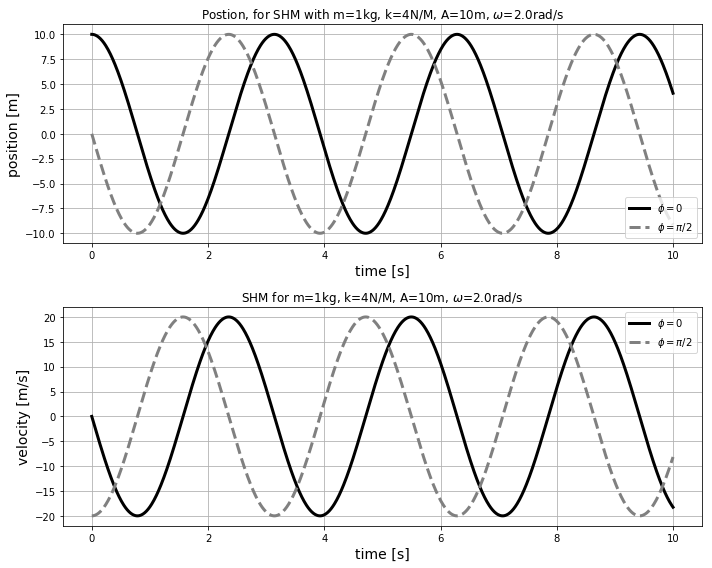
\includegraphics[width=0.9\linewidth]{files/xvtshm-68dd176ca6546f9b402443d7bc7befb2.png}
\caption[]{Position and velocity as a function of time for a mass-spring system for two different values of the phase, $\phi$.}
\label{fig:simpleharmonicmotion:xvtshm}
\end{figure}

We can make a few observations about the position and velocity illustrated in Figure~\ref{fig:simpleharmonicmotion:xvtshm}:

\begin{itemize}
\item Changing the phase, $\phi$, results in an horizontal shift of the functions. A positive phase results in a shift of the functions to the left.
\item The highest speed corresponds to a position of $x=0$ and the largest position, $x=\pm A$, corresponds to a speed of zero.
\item $\phi = 0$ corresponds to the ``initial condition'' at $t=0$, where the position of the mass is $x=A$ and its speed is $v=0$.
\item $\phi = \pi/2$ corresponds to the ``initial condition'' at $t=0$,  where the position of the mass is $x=0$ and its velocity is in the negative direction, and with maximal amplitude.
\item The position is always between $x=\pm A$, and the velocity is always between $v=\pm A\omega$.
\end{itemize}

The motion of the spring is clearly periodic. If the period of the motion is $T$, then the position of the mass at time $t$ will be the same as its position at $t+T$. The period of the motion, $T$, is easily found:
\begin{equation}
\boxed{T=\frac{2\pi}{\omega}=2\pi\sqrt{\frac{m}{k}}}
\end{equation}
And the corresponding frequency is given by:
\begin{equation}
\boxed{f = \frac{1}{T}=\frac{\omega}{2\pi}=\frac{1}{2\pi}\sqrt{\frac{k}{m}}}
\end{equation}
It should now be clear why $\omega$ is called the angular frequency, since it is related to the frequency of the motion.

\begin{framed}
\textbf{Checkpoint}\\
In order to double the oscillation period of a spring-mass system, you can

\begin{enumerate}
\item double the ratio of the mass over the spring constant.
\item quadruple the mass.
\item halve the spring constant.
\item All of the above.
\end{enumerate}

\begin{framed}
\textbf{Answer}\\
\begin{enumerate}[resume]
\item
\end{enumerate}
\end{framed}
\end{framed}

\paragraph{Analogy with uniform circular motion}

We can make an analogy between the mathematical description of the motion of a spring-mass system and that of uniform circular motion. Consider a particle that is moving along a circle of radius $A$, with constant angular speed $\omega$, as illustrated in Figure~\ref{fig:simpleharmonicmotion:circleshm}.

\begin{figure}[!htbp]
\centering
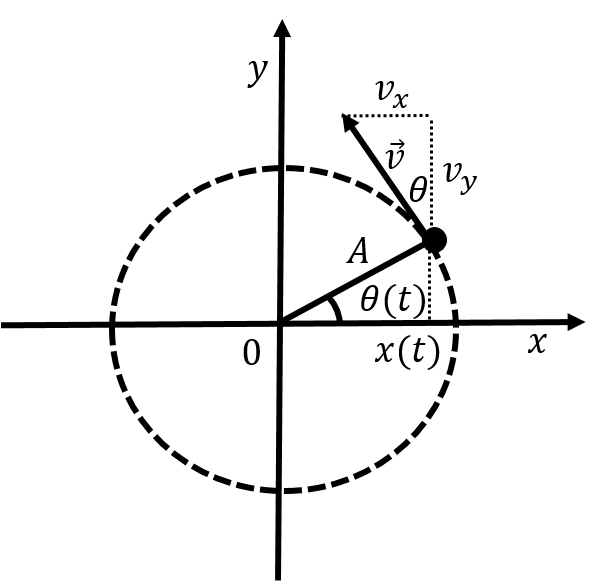
\includegraphics[width=0.4\linewidth]{files/circleshm-4fbc6d730682c8b2591f53fdde89cb8a.png}
\caption[]{Uniform circular motion of a particle along a circle of radius $A$ with constant angular speed $\omega$.}
\label{fig:simpleharmonicmotion:circleshm}
\end{figure}

The angular position, $\theta(t)$, of the particle is given by:
\begin{equation}
\theta(t) = \theta_0 + \omega t
\end{equation}
if the particle was located at an angular position $\theta_0$ at $t=0$ ($\theta_0=0$ in Figure~\ref{fig:simpleharmonicmotion:circleshm}). The $x$ coordinate of the particle is given by:
\begin{equation}
x(t) = A\cos(\theta(t)) = A\cos(\theta_0 + \omega t)
\end{equation}

We can see that the $x$ coordinate of the particle has the same functional form as the position for simple harmonic motion. The same is true for the particle's velocity. The magnitude of the particle's velocity is given by:
\begin{equation}
v = \omega r = \omega A
\end{equation}
where $r=A$ is the radius of the circle. The $x$ component of the particle's velocity is easily found from the figure and is given by:
\begin{equation}
v_x(t) = -v\sin(\theta(t)) = -\omega A\sin(\theta_0 + \omega t)
\end{equation}
We can visualize simple harmonic motion as if it were the projection onto the $x$ axis of uniform circular motion with angular speed $\omega$ about a circle with radius $A$. The phase $\phi$ corresponds to the angular position of the particle around the circle, $\theta_0$, at time $t=0$. When the particle crosses the $y$ axis ($x=0$), its velocity is in the $x$ direction, so the $x$ component of the velocity is maximal. When the particle crosses the $x$ axis ($x=\pm A$), the $x$ component of the velocity is zero.

\begin{framed}
\textbf{Olivia's Thoughts}\\
Here's a visualization of uniform circular motion projected onto the $x$ axis:

\begin{figure}[!htbp]
\centering
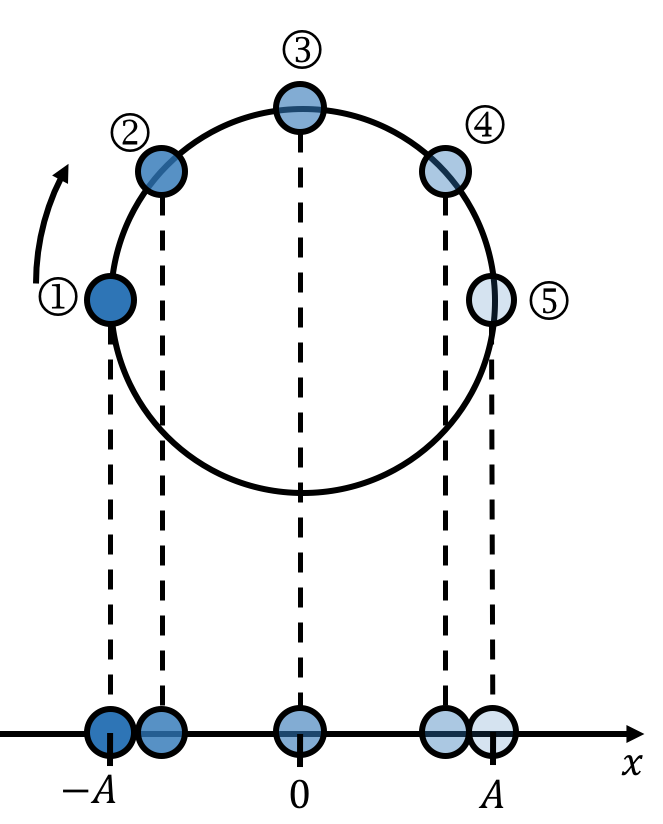
\includegraphics[width=0.4\linewidth]{files/circularmotionprojec-955ca62bb4a2c11eeccce046ef38be60.png}
\caption[]{Projecting the motion of a ball around a circle onto the $x$ axis.}
\label{fig:simpleharmonicmotion:projection}
\end{figure}

Figure~\ref{fig:simpleharmonicmotion:projection} shows a ball moving at a constant speed around a circle of radius $A$. In this diagram, I have taken snapshots of the ball's motion at regular time intervals as the ball moves from Position 1 to Position 5. Since the speed is constant, the balls are evenly spaced out around the circle. At the bottom of the figure, you can see what it would look like if we only considered the motion in the $x$ direction (this is the projection of the motion onto the $x$ axis). You could also think of this as what the motion would look like if you looked up at the circle from below. As you can see, this projection looks a lot like the motion of a mass on a spring. The motion of the ball is constrained between $-A$ and $+A$ (the turning points), and the velocity of the ball, in the $x$ direction, will be highest when $x=0$. There are tons of videos online that show animations of this concept, just look up ``SHM as a projection of circular motion'' and you will get lots of different ways to visualize this.
\end{framed}

\subsubsection{Vertical spring-mass system}

Consider the vertical spring-mass system illustrated in Figure~\ref{fig:simpleharmonicmotion:vertspring}.

\begin{figure}[!htbp]
\centering
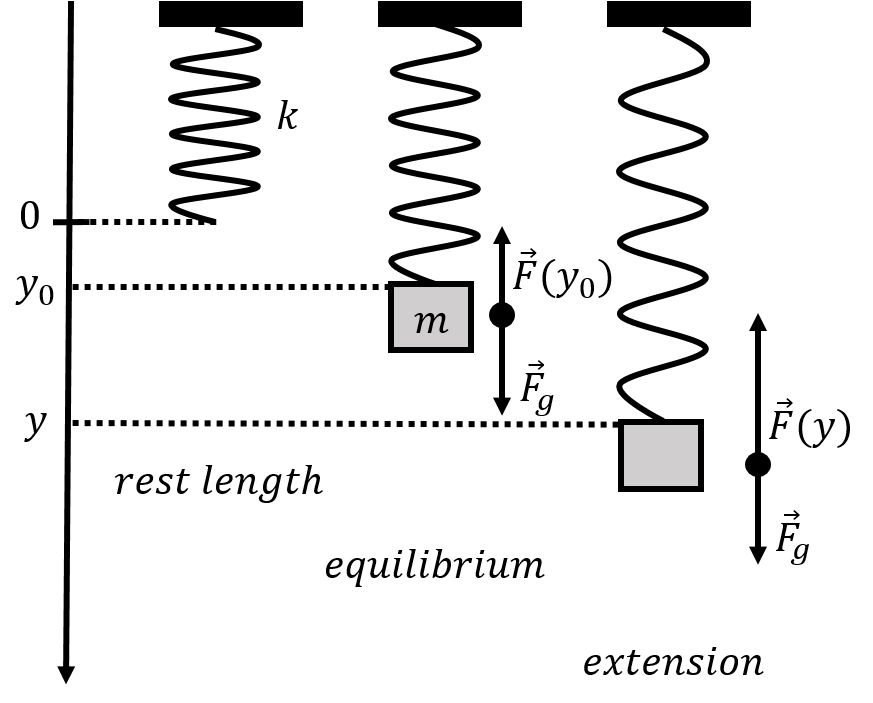
\includegraphics[width=0.5\linewidth]{files/vertspring-8534fbbc591565ea1db9f09dbdd7d36b.png}
\caption[]{A vertical spring-mass system.}
\label{fig:simpleharmonicmotion:vertspring}
\end{figure}

When no mass is attached to the spring, the spring is at rest (we assume that the spring has no mass). We choose the origin of a one-dimensional vertical coordinate system ($y$ axis) to be located at the rest length of the spring (left panel of Figure~\ref{fig:simpleharmonicmotion:vertspring}). When a mass $m$ is attached to the spring, the spring will extend  and the end of the spring will move to a new equilibrium position, $y_0$, given by the condition that the net force on the mass $m$ is zero. The only forces exerted on the mass are the force from the spring and its weight. The condition for the equilibrium is thus:
\begin{equation}
\sum F_y = F_g - F(y_0) &=0\\
 mg - ky_0 &= 0 \\
 \therefore mg &= ky_0
\end{equation}
Now, consider the forces on the mass at some position $y$ when the spring is extended downwards relative to the equilibrium position (right panel of Figure~\ref{fig:simpleharmonicmotion:vertspring}). Newton's Second Law at that position can be written as:
\begin{equation}
\sum F_y = mg - ky &= ma\\
\therefore m \frac{d^2y}{dt^2}& = mg - ky
\end{equation}
Note that the net force on the mass will always be in the direction so as to ``restore'' the position of the mass back to the equilibrium position, $y_0$. If the mass had been moved upwards relative to $y_0$, the net force would be downwards.

We can substitute the equilibrium condition, $mg = ky_0$, into the equation that we obtained from Newton's Second Law:
\begin{equation}
 m \frac{d^2y}{dt^2}& = mg - ky \\
m \frac{d^2y}{dt^2}&= ky_0 - ky\\
m \frac{d^2y}{dt^2}&=-k(y-y_0) \\
\therefore \frac{d^2y}{dt^2} &= -\frac{k}{m}(y-y_0)
\end{equation}
Consider a new variable, $y'=y -y_0$. This is the same as defining a new $y'$ axis that is shifted downwards by $y_0$; in other words, this the same as defining a new $y'$ axis whose origin is at $y_0$ (the equilibrium position) rather than at the position where the spring is at rest. Noting that the second time derivative of $y'(t)$ is the same as that for $y(t)$:
\begin{equation}
\frac{d^2y}{dt^2} &= \frac{d^2}{dt^2} (y' + y_0) = \frac{d^2y'}{dt^2}\\
\end{equation}
we can write the equation of motion for the mass, but using $y'(t)$ to describe its position:
\begin{equation}
\frac{d^2y'}{dt^2} &= -\frac{k}{m}y'
\end{equation}
This is the same equation as that for the simple harmonic motion of a horizontal spring-mass system (\ref{eq:simpleharmonicmotion:shmspring}), but with the \textbf{origin located at the equilibrium position} instead of at the rest length of the spring. In other words, a vertical spring-mass system will undergo simple harmonic motion in the vertical direction about the equilibrium position. In general, a spring-mass system will undergo simple harmonic motion if a constant force that is co-linear with the spring force is exerted on the mass (in this case, gravity). That motion will be centred about a point of equilibrium where the net force on the mass is zero rather than where the spring is at its rest position.

\begin{framed}
\textbf{Checkpoint}\\
How does the period of motion of a vertical spring-mass system compare to the period of a horizontal system (assuming the mass and spring constant are the same)?

\begin{enumerate}
\item The period of the vertical system will be larger.
\item The period of the vertical system will be smaller.
\item The period will be the same.
\end{enumerate}

\begin{framed}
\textbf{Answer}\\
\begin{enumerate}[resume]
\item
\end{enumerate}
\end{framed}
\end{framed}

\paragraph{Two-spring-mass system}

Consider a horizontal spring-mass system composed of a single mass, $m$, attached to two different springs with spring constants $k_1$ and $k_2$, as shown in Figure~\ref{fig:simpleharmonicmotion:2springs}.

\begin{figure}[!htbp]
\centering
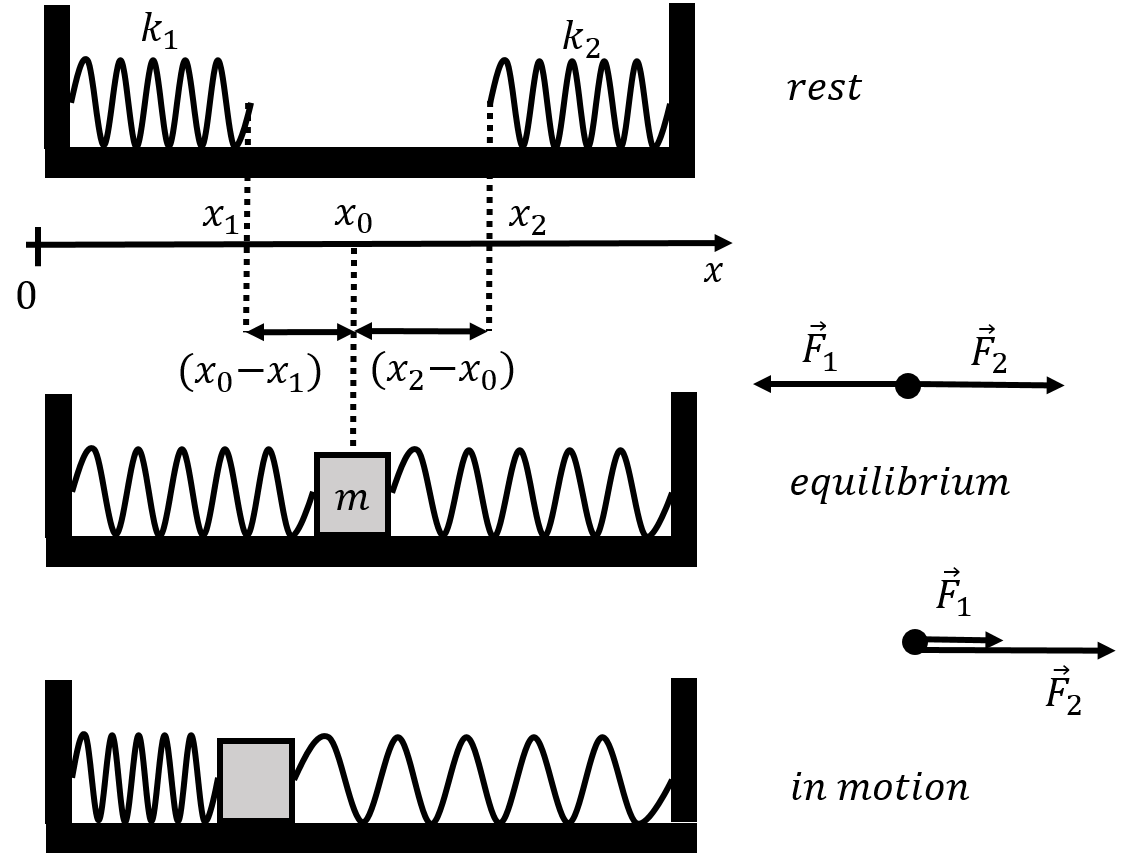
\includegraphics[width=0.7\linewidth]{files/2springs-036a2db7121c1ee98e916eb5709b95e1.png}
\caption[]{A mass attached to two different springs.}
\label{fig:simpleharmonicmotion:2springs}
\end{figure}

We introduce a horizontal coordinate system, such that the end of the spring with spring constant $k_1$ is at position $x_1$ when it is at rest, and the end of the $k_2$ spring is at $x_2$ when it is as rest, as shown in the top panel. A mass $m$ is then attached to the two springs, and $x_0$ corresponds to the equilibrium position of the mass when the net force from the two springs is zero. We will assume that the length of the mass is negligible, so that the ends of both springs are also at position $x_0$ at equilibrium. You can see in the middle panel of Figure~\ref{fig:simpleharmonicmotion:2springs} that both springs are in extension when in the equilibrium position. It is possible to have an equilibrium where both springs are in compression, if both springs are long enough to extend past $x_0$ when they are at rest.

If we assume that both springs are in extension at equilibrium, as shown in the figure, then the condition for equilibrium is given by requiring that the sum of the forces on the mass is zero when the mass is located at $x_0$. The extension of the spring on the left is $x_0 - x_1$, and the extension of the spring on the right is $x_2 -x_0$:
\begin{equation}
\sum F_x = -k_1(x_0-x_1) + k_2 (x_2 - x_0) &= 0\\
-k_1x_0+k_1x_1+k_2x_2-k_2x_0 &=0\\
-(k_1+k_2)x_0 +k_1x_1+k_2x_2 &=0\\
\therefore k_1x_1+k_2x_2 &=(k_1+k_2)x_0
\end{equation}
Note that if the mass is displaced from $x_0$ in any direction, the net force on the mass will be in the direction of the equilibrium position, and will act to ``restore'' the position of the mass back to $x_0$.

When the mass is at some position $x$, as shown in the bottom panel (for the $k_1$ spring in compression and the $k_2$ spring in extension), Newton's Second Law for the mass is:
\begin{equation}
-k_1(x-x_1) + k_2 (x_2 - x) &= m a \\
-k_1x +k_1x_1 + k_2 x_2 - k_2 x &= m \frac{d^2x}{dt^2}\\
-(k_1+k_2)x  + k_1x_1 + k_2 x_2&= m \frac{d^2x}{dt^2}
\end{equation}
Note that, mathematically, this equation is of the form $-kx + C =ma$, which is the same form of the equation that we had for the vertical spring-mass system (with $C=mg$), so we expect that this will also lead to simple harmonic motion. We can use the equilibrium condition ($k_1x_1+k_2x_2 =(k_1+k_2)x_0$) to re-write this equation:
\begin{equation}
-(k_1+k_2)x  + k_1x_1 + k_2 x_2&= m \frac{d^2x}{dt^2}\\
-(k_1+k_2)x  + (k_1+k_2)x_0&= m \frac{d^2x}{dt^2}\\
\therefore -(k_1+k_2) (x-x_0) &= m \frac{d^2x}{dt^2}
\end{equation}
Let us define $k=k_1+k_2$ as the ``effective'' spring constant from the two springs combined. We can also define a new coordinate, $x' = x -x_0$, which simply corresponds to a new $x$ axis whose origin is located at the equilibrium position (in a way that is exactly analogous to what we did in the vertical spring-mass system). We can thus write Newton's Second Law as:
\begin{equation}
-(k_1+k_2) (x-x_0) &= m \frac{d^2x}{dt^2}\\
 -kx' &= m \frac{d^2x'}{dt^2}\\
 \therefore \frac{d^2x'}{dt^2} &= -\frac{k}{m}x'
\end{equation}
and we find that the motion of the mass attached to two springs is described by the same equation of motion for simple harmonic motion as that of a mass attached to a single spring. In this case, the mass will oscillate about the equilibrium position, $x_0$, with a an effective spring constant $k=k_1+k_2$. Combining the two springs in this way is thus equivalent to having a single spring, but with spring constant $k=k_1+k_2$. The angular frequency of the oscillations is given by:
\begin{equation}
\omega = \sqrt{\frac{k}{m}}=\sqrt{\frac{k_1+k_2}{m}}
\end{equation}

\subsubsection{Simple harmonic motion}

In the previous sections, we modelled the motion of a mass attached to a spring and found that its position, $x(t)$, was described by the following differential equation:
\begin{equation}
\label{eq:simpleharmonicmotion:shm}
\boxed{\frac{d^2x}{dt} = -\omega^2x}
\end{equation}
A possible solution to that equation was given by:
\begin{equation}
\label{eq:simpleharmonicmotion:shmsol}
\boxed{x(t) = A\cos(\omega t+ \phi)}
\end{equation}
We then saw that the motion of a vertical spring-mass system, as well as that of a mass attached to two springs, could also be described by (\ref{eq:simpleharmonicmotion:shm}). Any physical system that can described by (\ref{eq:simpleharmonicmotion:shm}) is said to undergo ``simple harmonic motion'', or to be a ``simple harmonic oscillator''. If we find that the physical model of a system leads to (\ref{eq:simpleharmonicmotion:shm}), then we immediately know that the position of system can be described by (\ref{eq:simpleharmonicmotion:shmsol}).

The key physical characteristic of a simple harmonic oscillator is that there is a ``restoring force'' whose magnitude is proportional to the displacement from the equilibrium position. A restoring force is a force that acts to place the system back in equilibrium, and is thus always in the direction that is opposite of the displacement relative to an equilibrium position. In the three systems that we considered so far, the net force on the mass was always such that it would restore the mass back to the equilibrium position, where the net force on the mass is zero.

Many systems in nature are well modelled as simple harmonic oscillators. Some examples are: the motion of a pendulum as it oscillates, the motion of a buoy bobbing up and down in the sea, the motion of electrons in a shorted capacitor, and the vibrations of atoms in a molecule.

\subsubsection{The motion of a pendulum}

In this section, we show how and when the motion of a pendulum can be described as simple harmonic motion. Consider the simple pendulum that is constructed from a mass-less string of length, $L$, attached to a fixed point on one end and to a point mass $m$ on the other, as illustrated in Figure~\ref{fig:simpleharmonicmotion:simplep}.

\begin{figure}[!htbp]
\centering
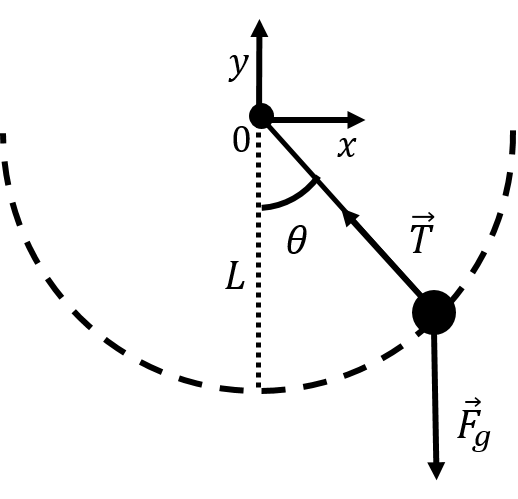
\includegraphics[width=0.3\linewidth]{files/simplep-b3f8d339f98d4ddd93972dc7996f4e89.png}
\caption[]{A simple pendulum which oscillates in a vertical plane.}
\label{fig:simpleharmonicmotion:simplep}
\end{figure}

The pendulum can swing in the vertical plane, and we have shown our choice of coordinate system (the $z$ axis, not shown, is out of the page). The only two forces on the mass are the tension from the string and its weight. We can describe the position of the mass by the angle, $\theta(t)$, that the string makes with the vertical. We can model the dynamics of the simple pendulum by considering the net torque and angular acceleration about the axis of rotation that is perpendicular to the plane of the page and that goes through the point on the string that is fixed.

The force of tension cannot create a torque on the mass about the axis of rotation, as it is anti-parallel to the vector from the point of rotation to the mass. The net torque is thus the torque from the force of gravity:
\begin{equation}
\vec\tau^{net} &=\vec \tau_g \\
&=\vec r \times \vec F_g = (L\sin\theta \hat x - L\cos\theta \hat y) \times (-mg\hat y)\\
&=-mgL\sin\theta \hat z
\end{equation}
where $L$ is the magnitude of the vector, $\vec r$, from the axis of rotation to where the force of gravity is exerted. The net torque is equal to the angular acceleration, $\alpha$, multiplied by the moment of inertia, $I$, of the mass:
\begin{equation}
\vec\tau^{net} &= I\vec\alpha\\
-mgL\sin\theta \hat z&= mL^2 \vec\alpha\\
-g\sin\theta \hat z&= L \vec\alpha
\end{equation}
where $I=ML^2$ is the moment of inertia for a point mass a distance $L$ away from the axis of rotation. For the position illustrated in Figure~\ref{fig:simpleharmonicmotion:simplep}, the angular acceleration of the pendulum is in the negative $z$ direction (into the page) and corresponds to a clockwise motion for the pendulum, as we would expect. The angular acceleration is the second time derivative of the angle, $\theta$:
\begin{equation}
\alpha = \frac{d^2\theta}{dt^2}
\end{equation}
We can thus re-write the equation that we obtained from the rotational dynamics version of Newton's Second Law as:
\begin{equation}
-g\sin\theta \hat z&= L \vec\alpha\\
\frac{d^2\theta}{dt^2} &= -\frac{g}{L}\sin\theta
\end{equation}
where we only used the magnitudes in the second equation, since all of the angular quantities are in the $z$ direction. This equation of motion for $\theta(t)$ almost looks like the equation for simple harmonic oscillation for the angle $\theta$ (except that we have $\sin\theta$ instead of $\theta$). However, consider the ``the small angle approximation''{\textbackslash}footnote\{Look up the Maclaurin/Taylor series for the sine function!\} for the sine function:
\begin{equation}
\sin\theta \approx \theta
\end{equation}
If the oscillations of the pendulum are ``small'', such that the small angle approximation is valid, then the equation of motion for the pendulum is:
\begin{equation}
\frac{d^2\theta}{dt^2} &= -\frac{g}{L}\sin\theta \approx -\frac{g}{L}\theta \\
\therefore \frac{d^2\theta}{dt^2} &=-\frac{g}{L}\theta \quad (\text{for small }\theta)
\end{equation}
and the angle that the pendulum makes with the vertical is described by the equation for simple harmonic oscillation with angular frequency:
\begin{equation}
\omega = \sqrt{\frac{g}{L}}
\end{equation}
The angle, $\theta$, as a function of time is thus described by the function:
\begin{equation}
\theta(t) = \theta_{max}\cos(\omega t +\phi)
\end{equation}
where $\theta_{max}$ is the maximal amplitude of the oscillations and $\phi$ is a phase that depends on when we choose to define $t=0$.

\begin{framed}
\textbf{Checkpoint}\\
Kaiden built a grandfather clock using a simple pendulum, but he found that the period was twice as large as as he wanted it to be. In order to halve the period of the pendulum, he can

\begin{enumerate}
\item change the mass.
\item halve the length of the string.
\item quarter the length of the string.
\item double the length of the string.
\item quadruple the length of the string.
\end{enumerate}

\begin{framed}
\textbf{Answer}\\
\begin{enumerate}[resume]
\item
\end{enumerate}
\end{framed}
\end{framed}

\paragraph{The physical pendulum}

A physical pendulum is defined as any object that is allowed to rotate in the vertical plane about some axis that goes through the object, as illustrated in Figure~\ref{fig:simpleharmonicmotion:physicalp}.

\begin{figure}[!htbp]
\centering
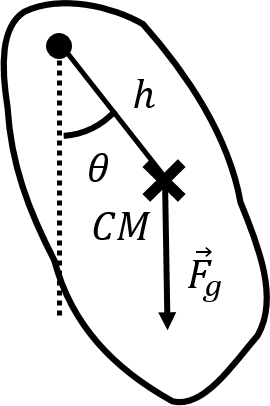
\includegraphics[width=0.2\linewidth]{files/physicalp-bd5a3302cad14b4ec3a2bf76983fb9cb.png}
\caption[]{A physical pendulum which oscillates in a vertical plane about an axis through the object.}
\label{fig:simpleharmonicmotion:physicalp}
\end{figure}

The only forces exerted on the pendulum are its weight (exerted at its centre of mass) and a contact force exerted at the axis of rotation. The physical pendulum can be modelled in exactly the same way as the simple pendulum, except that we use the moment of inertia of the object about the axis of rotation. Only the weight results in a torque about the rotation axis, since the contact force is exerted at the rotation axis:
\begin{equation}
\tau^{net} = \tau_g &= I\alpha\\
-mgh\sin\theta &= I\alpha = I \frac{d^2\theta}{dt^2}
\end{equation}
where $h$ is the distance from the axis of rotation to the centre of mass. In the small angle approximation, this becomes:
\begin{equation}
\frac{d^2\theta}{dt^2} &=-\frac{mgh}{I}\theta \quad (\text{for small }\theta)
\end{equation}
and we find that the physical pendulum oscillates with an angular frequency:
\begin{equation}
\omega = \sqrt{\frac{mgh}{I}}
\end{equation}

\subsubsection{Summary}

The equation of motion for the position, $x(t)$, of the mass in a one-dimensional spring-mass system with no friction can be written:
\begin{equation}
\frac{d^2x}{dt^2}=-\frac{k}{m}x = -\omega^2 x
\end{equation}
and has a solution:
\begin{equation}
x(t) = A\cos(\omega t + \phi)
\end{equation}
where $A$ is the amplitude of the motion, $\phi$ is the phase, which depends on our choice of initial conditions (when we choose time $t=0$), and $\omega$:
\begin{equation}
\omega = \sqrt{\frac{k}{m}}
\end{equation}
is the angular frequency of the motion. The mass will oscillate about an equilibrium position with a period, $T$, and frequency, $f$, given by:
\begin{equation}
T&=\frac{2\pi}{\omega}=2\pi\sqrt{\frac{m}{k}}\\
f&=\frac{1}{T}=\frac{\omega}{2\pi}=\frac{1}{2\pi}\sqrt{\frac{k}{m}}
\end{equation}
The velocity and acceleration of the mass are found by taking the time derivatives of the position $x(t)$:
\begin{equation}
x(t)&= A \cos(\omega t + \phi)\\
v(t)&=\frac{d}{dt}x(t) = -A\omega\sin(\omega t + \phi)\\
a(t)&= \frac{d^2}{dt^2}x(t) =\frac{d}{dt}\left( -A\omega\sin(\omega t + \phi)\right)= -A\omega^2\cos(\omega t + \phi)
\end{equation}
The total mechanical energy of the mass, at some position $x$, is given by:
\begin{equation}
E =U+K=\frac{1}{2}kx^2+\frac{1}{2}mv^2= \frac{1}{2}kA^2
\end{equation}
and is conserved.

Any system that can be described by the equation of motion:
\begin{equation}
\frac{d^2x}{dt^2}= -\omega^2 x
\end{equation}
is said to be a simple harmonic oscillator, and its position will be described by:
\begin{equation}
x(t) = A\cos(\omega t + \phi)
\end{equation}
A simple harmonic oscillator will always oscillate about an equilibrium position, where the net force on the oscillator is zero. The net force on a simple harmonic oscillator is always directed towards the equilibrium position, and has a magnitude proportional to the distance of the oscillator from its equilibrium position. The force is called a restoring force. A vertical spring-mass system, and a mass attached to two springs will both undergo simple harmonic motion about their respective equilibrium position.

A simple pendulum will undergo simple harmonic oscillations, if the amplitude of the oscillations is small. The angular frequency for the oscillations of a simple pendulum only depends on the length of the pendulum:
\begin{equation}
\omega = \sqrt{\frac{g}{L}}
\end{equation}
This is valid in the small angle approximation, where:
\begin{equation}
\sin\theta \approx \theta
\end{equation}
A physical pendulum of mass $m$ which oscillates about an axis through the object will also undergo simple harmonic oscillation in the small angle approximation. The angular frequency of the oscillations for a physical pendulum is given by:
\begin{equation}
\omega = \sqrt{\frac{mgh}{I}}
\end{equation}
where $h$ is the distance between the centre of mass and the axis of rotation, and $I$ is the moment of inertia of the object about the rotation axis.

\begin{framed}
\textbf{Important Equations}\\
\textbf{Position, velocity, and {\textbackslash}acceleration for SHM:}
\begin{equation}
x(t)&= A \cos(\omega t + \phi)\\
v(t)&=\frac{d}{dt}x(t) = -A\omega\sin(\omega t + \phi)\\
a(t)&= \frac{d^2}{dt^2}x(t) = -A\omega^2\cos(\omega t + \phi)
\end{equation}
\textbf{Period and frequency:}
\begin{equation}
\omega &= \sqrt{\frac{k}{m}}\\
T&=\frac{2\pi}{\omega}=2\pi\sqrt{\frac{m}{k}}\\
f&=\frac{1}{T}=\frac{\omega}{2\pi}=\frac{1}{2\pi}\sqrt{\frac{k}{m}}
\end{equation}
\textbf{Mechanical energy:}
\begin{equation}
E =U+K=\frac{1}{2}kx^2+\frac{1}{2}mv^2= \frac{1}{2}kA^2
\end{equation}
\textbf{Simple pendulum (small angles):}
\begin{equation}
\omega = \sqrt{\frac{g}{L}}
\end{equation}
\textbf{Physical pendulum (small angles):}
\begin{equation}
\omega = \sqrt{\frac{mgh}{I}}
\end{equation}
\end{framed}

\begin{framed}
\textbf{Important Definitions}\\
\begin{itemize}
\item \textbf{Angular frequency:} is related to a usual frequency by a factor of $2\pi$. For an object rotating around a circle at constant speed, the angular frequency of the rotation is the same as the angular speed (the rate of change of a position angle). SI units: [${\rm rad/s}$]. Common variable(s): $\omega$.
\end{itemize}
\end{framed}

\subsubsection{Thinking about the material}

\begin{framed}
\textbf{Reflect and research}\\
\begin{itemize}
\item What is an example of a system that is a simple harmonic oscillator (not covered in this this chapter)? What is the restoring force for that system?
\item What happens to the motion of a mass-spring system in the presence of friction? Sketch out the position as a function of time.
\item What is a ``damped'' harmonic oscillator?
\item What is a coupled oscillator? Find a video of a coupled oscillator online and describe the motion.
\item How do the shock absorbers on a car relate to simple harmonic motion?
\end{itemize}
\end{framed}

\begin{framed}
\textbf{To try at home}\\
\begin{itemize}
\item Compare values of $\theta$ and $\sin\theta$ to see when the small angle approximation holds. Does it matter if $\theta$ is expressed in radians?
\item Build a simple pendulum and describe the motion. Is it simple harmonic motion? Is it damped simple harmonic motion? Does the frequency depend on the length of the pendulum as expected?
\end{itemize}
\end{framed}

\begin{framed}
\textbf{To try in the lab}\\
\begin{itemize}
\item Theory lab: what is the function $x(t)$ if there is a frictional force, proportional to velocity, $-bv$, exerted on the spring mass system?
\item Propose an experiment to test whether the period of the motion of pendulum depends on the amplitude of the motion.
\item Propose an experiment to test whether a physical pendulum is well-described by simple harmonic motion.
\item 
\item Propose an experiment which measures the gravitational constant ($G$) using a torsion pendulum.
\end{itemize}
\end{framed}

\subsubsection{Sample problems and solutions}

\paragraph{Problems}

\begin{framed}
\textbf{Problem 12.1}\\
Ty ($m=30 {\rm kg}$) is trying out a new piece of equipment at his local playground. The equipment consists of a platform that is connected to two springs. The top spring ($k_1=2400 {\rm N/m}$) connects the platform to the playground structure and the bottom spring ($k_2=3480 {\rm N/m}$) (Figure~\ref{fig:simpleharmonicmotion:playground}) connects it to the ground. When no one is standing on the platform the platform is $50 {\rm cm}$ off the ground. When Ty is standing on the platform, he oscillates up and down, and the lowest point that the platform reaches is $35 {\rm cm}$ off the ground. Show that this is simple harmonic motion and determine what Ty's maximum speed will be.

\begin{figure}[!htbp]
\centering
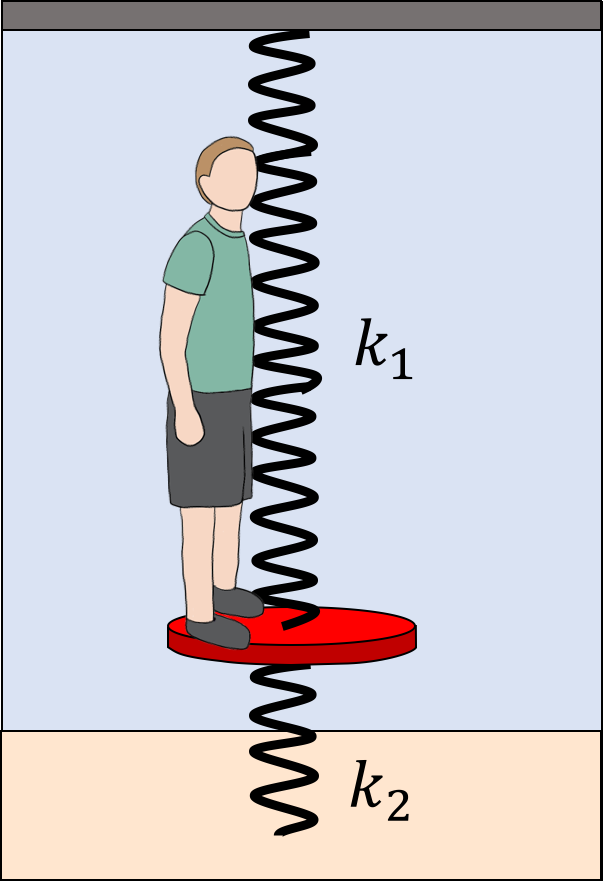
\includegraphics[width=0.3\linewidth]{files/playground1-99f6e4f872192288a95a159682b17661.png}
\caption[]{Playground equipment made of a platform connected to two vertical springs.}
\label{fig:simpleharmonicmotion:playground}
\end{figure}
\end{framed}

\begin{framed}
\textbf{Problem 12.2}\\
A torsional pendulum consists of a horizontal rod suspended from a vertical wire. When the rod is rotated so that it is displaced an angle $\theta$ from equilibrium, the wire (which is now twisted) provides a restoring torque about the axis of the wire given by:
\begin{equation}
\tau=-\kappa\theta
\end{equation}
where $\kappa$ is the torsion coefficient, which depends on the stiffness of the wire. You may notice that this formula closely resembles Hooke's law.

\begin{itemize}
\item a.  You construct a torsional pendulum by attaching two small spherical masses (you can assume they are point masses, each of mass $m$) to the ends of a thin (mass-less) rod of length $L$ and attaching a wire to the centre of the rod (Figure~\ref{fig:simpleharmonicmotion:torsional1}). When you displace one of the masses by an angle $\theta$ and release it, you find that it oscillates with a period $T$. Find an expression for the torsion coefficient, $\kappa$, in term of $T$, $m$, and $L$.
\end{itemize}

\begin{figure}[!htbp]
\centering
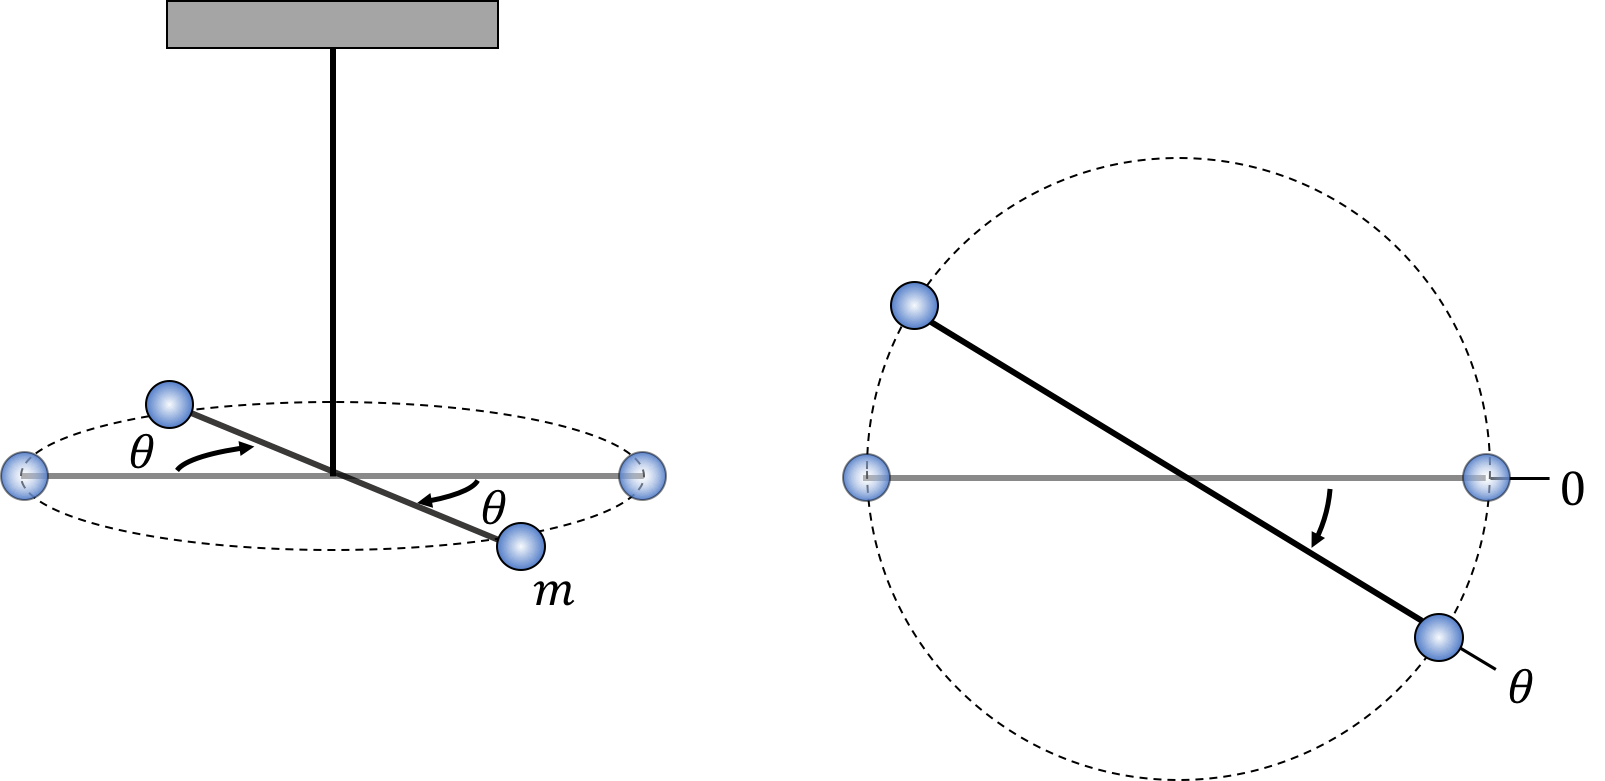
\includegraphics[width=0.8\linewidth]{files/torsionalpendulum1-1a91cb49135990459b6e33c6b4b493fc.png}
\caption[]{A torsional pendulum. The right side shows a top view.}
\label{fig:simpleharmonicmotion:torsional1}
\end{figure}

\begin{itemize}
\item b. You place two very large spheres, each of mass $M$, near each of the small spheres (as shown in Figure~\ref{fig:simpleharmonicmotion:torsional2}). Each of the small spheres will be acted on by a force of gravity from the \textbf{nearest} large sphere. The pendulum is at equilibrium when it is deflected an angle $\beta$ from its original equilibrium position. At the new equilibrium, the displacement vectors connecting the centres of large and small spheres have a magnitude $d$ and are essentially perpendicular to the rod. Find an expression for the universal gravitational constant $G$, in terms of the masses, the length of the rod, and the period measured in part a).
\end{itemize}

Fun fact! This set-up resembles an experiment performed by Henry Cavendish that was first used to determine the value for $G$ and to test Newton's Universal Theory of Gravity.

\begin{figure}[!htbp]
\centering
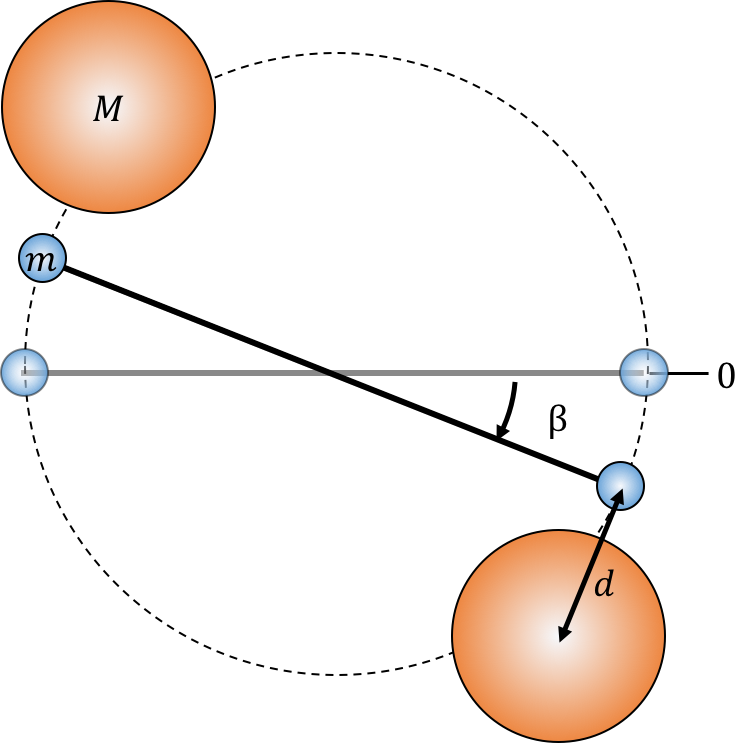
\includegraphics[width=0.4\linewidth]{files/torsionalpendulum2-ff2f313312974ebee0e8d1ecd462646c.png}
\caption[]{Two very large spheres are placed near each of the small masses on the torsional pendulum (top view). At the new equilibrium, each small mass is a distance $d$ from the nearest large mass.}
\label{fig:simpleharmonicmotion:torsional2}
\end{figure}
\end{framed}

\paragraph{Solutions}

\begin{framed}
\textbf{Solution 12.1}\\
First, we need to solve for the new equilibrium position of the platform, $x_0$, when Ty is standing on the platform. We define the $x$ axis so that the origin is $50 {\rm cm}$ above the ground (the equilibrium position when no one is standing on the platform) and choose the positive direction to be downwards (Figure~\ref{fig:simpleharmonicmotion:playground2}).

\begin{figure}[!htbp]
\centering
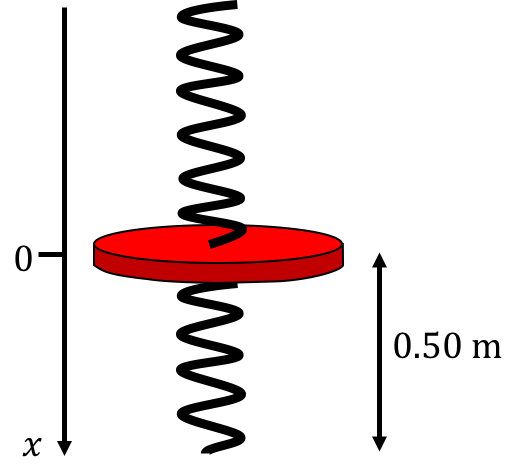
\includegraphics[width=0.35\linewidth]{files/playground2-736b77ec8dd366bba14b67d50562b83e.png}
\caption[]{The platform when no one is standing on it.}
\label{fig:simpleharmonicmotion:playground2}
\end{figure}

Even though we do not know the mass of the platform, or the actual resting lengths of the spring, we do not need to know these, since we can model the platform with nobody on it as a single spring with spring constant $k=k_1+k_2$ and rest position $x=0$.

When Ty is standing on the platform, the sum of the forces is given by his weight and the force from the ``effective spring'':
\begin{equation}
\sum F=mg-(k_1+k_2)x
\end{equation}
where we noted that, when the platform moves down, both the top and bottom spring will exert a force upwards (Figure~\ref{fig:simpleharmonicmotion:playgroundfbd}).

At equilibrium, the sum of the forces is equal to zero. We can use this to solve for the displacement at $x_0$:
\begin{equation}
0&=mg-(k_1+k_2)x_0\\
\therefore x_0&=\frac{mg}{k_1+k_2}=\frac{(30 {\rm kg})(9.8 {\rm m/s^2})}{(2400 {\rm Nm})+(3480 {\rm Nm})}=0.05 {\rm m}
\end{equation}
We will confirm that this is a simple harmonic oscillator by showing that the system's motion can be described by the equation:
\begin{equation}
\frac{d^2x}{dt^2}&=-\omega^2x
\end{equation}
For some position $x$ below equilibrium, we can rewrite Newton's second law as:
\begin{equation}
ma&=mg-(k_1+k_2)x\\
m\frac{d^2x}{dt^2}&=mg-(k_1+k_2)x
\end{equation}
In order to show that this is simple harmonic motion, we need to combine the right hand side of the equation into one term. We found earlier that $mg=(k_1+k_2)x_0$, which we can use here:
\begin{equation}
m\frac{d^2x}{dt^2}&=(k_1+k_2)x_0-(k_1+k_2)x\\
\frac{d^2x}{dt^2}&=\frac{(k_1+k_2)}{m}(x_0-x)\\
\frac{d^2x}{dt^2}&=-\frac{(k_1+k_2)}{m}(x-x_0)\\
\end{equation}
We now define an $x'$ axis such that $x'=x -x_0$. This means that the origin of the $x'$ axis is at the new equilibrium position:

\begin{figure}[!htbp]
\centering
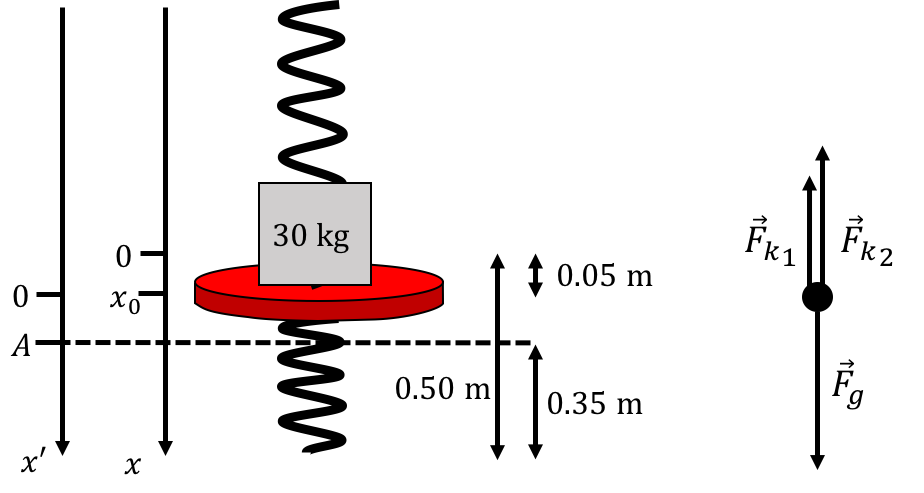
\includegraphics[width=0.7\linewidth]{files/playgroundfbd-7e3f532fe4d4cba994b3fd3729e258ee.png}
\caption[]{The forces acting on the platform and our new coordinate system.}
\label{fig:simpleharmonicmotion:playgroundfbd}
\end{figure}

We can now rewrite our expression using the $x'$ axis:
\begin{equation}
\frac{d^2x}{dt^2}&=-\frac{(k_1+k_2)}{m}x'
\end{equation}
This equation tells us that this is simple harmonic motion about the new equilibrium position, where $\omega=\sqrt{(k_1+k_2)/m}$. We know that the lowest point that the platform reaches is $35 {\rm cm}$ above the ground, which, on our $x'$ axis, corresponds to $x'=10 {\rm cm}$ (Figure~\ref{fig:simpleharmonicmotion:playgroundfbd}). Thus, the amplitude of the oscillation is $A=0.1 {\rm m}$. Because this is simple harmonic motion, we know that the position of the platform can be described by the following function:
\begin{equation}
x'(t)&= A \cos(\omega t + \phi)
\end{equation}
We set $t=0$ to be when the platform is at its lowest point ($x'=A$). The value of $\phi$ is thus:
\begin{equation}
x'(0)&= A \cos(\omega (0) + \phi)\\
A&= A \cos(\phi)\\
1&=\cos(\phi)\\
\therefore \phi&=0
\end{equation}
The velocity is given by:
\begin{equation}
v(t)=\frac{d}{dt}x(t) &= -A\omega\sin(\omega t + \phi)\\
&=-A\omega\sin(\omega t)
\end{equation}
The speed will be maximized when $\sin(\omega t)=1\quad \textrm{or} -1$ . So, the maximum speed will be:
\begin{equation}
|v|&=A\omega\\
|v|&=A\sqrt{\frac{(k_1+k_2)}{m}}\\
|v|&=(0.1 {\rm m})\sqrt{\frac{(2400 {\rm Nm}+3480 {\rm Nm})}{30 {\rm kg}}}\\
|v|&=1.4 {\rm m/s}
\end{equation}
\end{framed}

\begin{framed}
\textbf{Solution 12.2}\\
\begin{itemize}
\item a. The only force that creates a torque on the masses is the restoring force from the twisting of the wire. The rotational dynamics version of Newton's Second Law relates this torque to the angular acceleration, $\alpha$ of the rod:
\end{itemize}
\begin{equation}
I\alpha=-\kappa\theta
\end{equation}
where $I$ is the moment of inertia of the rod. Rewriting $\alpha$ more explicitly as the second time derivative of the angle, we get:
\begin{equation}
I\frac{d^2\theta}{dt^2}&=-\kappa\theta\\
\frac{d^2\theta}{dt^2}&=-\frac{\kappa}{I}\theta\\
\end{equation}
By inspection, we can see that the torsional pendulum is a simple harmonic oscillator, where $\omega=\sqrt{\kappa/I}$. The period of the motion is therefore:
\begin{equation}
T&=\frac{2\pi}{\omega}\\
T&=2\pi\sqrt{\frac{I}{\kappa}}
\end{equation}
We can rearrange this expression to get $\kappa$:
\begin{equation}
T^2&=\frac{4\pi^2I}{\kappa}\\
\kappa&=\frac{4\pi^2I}{T^2}
\end{equation}
The moment of inertia for one of the masses is $m(L/2)^2$, where $L/2$ is the distance from the mass to the axis of rotation. The moment of inertia for the two masses attached to the mass-less rod is:
\begin{equation}
I&=2m\left(\frac{L}{2}\right)^2=\frac{mL^2}{2}\\
\end{equation}
Putting this into our expression for $\kappa$:
\begin{equation}
\kappa=\frac{2\pi^2mL^2}{T^2}
\end{equation}
\begin{itemize}
\item b. The two forces that provide torques for the small spheres are gravity and the force exerted by the twisting wire. Each of the small spheres will experience a force due to gravity from the nearest large sphere. At equilibrium, the force due to gravity on one of the small spheres is therefore:
\end{itemize}
\begin{equation}
F_g=\frac{GMm}{d^2}
\end{equation}
Assuming that, at equilibrium, the force vector is perpendicular to the rod, the torque from one of the large spheres is just the force multiplied by the distance to the axis of rotation. Since there are two large spheres, each of which creates a torque on the pendulum, the total torque due to gravity is:
\begin{equation}
\tau_g&=2F_g\frac{L}{2}\\
&=F_gL\\
&=\frac{GMm}{d^2}L
\end{equation}
(Note that $\tau g$ is the torque due to gravity \textbf{at equilibrium only}). We can use Newton's second law for the pendulum to find an expression for $G$. At equilibrium, the net torque is equal to zero, and the angle of deflection is $\beta$:
\begin{equation}
\tau_{net}&=\tau_{wire}-\tau_g\\
0&=\tau_{wire}-\tau_g\\
\tau_g&=\tau_{wire}\\
\frac{GMm}{d^2}L&=\kappa\beta\\
\therefore G&=\frac{\kappa\beta d^2}{LMm}
\end{equation}
Using our expression for $\kappa$ found in part a), this becomes:
\begin{equation}
G=\frac{2\pi^2L\beta d^2}{MT^2}
\end{equation}
\end{framed}